
\usepackage[T1]{fontenc}
\usepackage[utf8]{inputenc}
\usepackage{lmodern}
\usepackage{babel}
\usepackage{listings}
\usepackage{color}
\usepackage{tabularx}
\usepackage{textpos}
\usepackage{wallpaper}
\usepackage{pgfpages}
\usepackage{etoolbox} % to setup lstinputlisting
\usepackage{dirtytalk}
\usepackage{epigraph}

% settings to draw border around every first 3 slide per sheet
\pgfpageslogicalpageoptions{1}{border code=\pgfusepath{stroke}}
\pgfpageslogicalpageoptions{2}{border code=\pgfusepath{stroke}}
\pgfpageslogicalpageoptions{3}{border code=\pgfusepath{stroke}}

\setcounter{tocdepth}{1}

\definecolor{pythoncommentcolor}{rgb}{0,0.6,0}
\definecolor{linenumbercolor}{rgb}{0.5,0.5,0.5}
\definecolor{pythonstringcolor}{rgb}{0.58,0,0.82}
\definecolor{codebackgroundcolor}{rgb}{0.95,0.95,1}
\definecolor{outputbackgroundcolor}{rgb}{0.95,0.95,0.95}

\setlength{\epigraphwidth}{0.9\textwidth}

% Define styles for listing package
\lstdefinestyle{pythoncode}{
	backgroundcolor=\color{codebackgroundcolor}, % choose the background color
	basicstyle=\footnotesize\ttfamily, % the size of the fonts that are used for the code 
	language=Python, 
	commentstyle=\color{pythoncommentcolor},
	breaklines=true, % sets automatic line breaking
	captionpos=b, % sets the caption-position to bottom
	keywordstyle=\color{blue},
	stringstyle=\color{pythonstringcolor},
	numbers=left, % where to put the line-numbers
	numbersep=5pt, % how far the line-numbers are from the code
	numberstyle=\tiny\color{linenumbercolor},
	stepnumber=1, % the step between two line-numbers. If it's 1, each line will be numbered
	tabsize=4, % sets default tabsize to 4 spaces
	title=\lstname, % show the filename of files included with \lstinputlisting; also try caption instead of title
	showstringspaces=false % no special string spaces
}
\lstdefinestyle{pythonoutput}{
	backgroundcolor=\color{outputbackgroundcolor}, % choose the background color
	basicstyle=\footnotesize\ttfamily, % the size of the fonts that are used for the code 
	aboveskip=-20pt
}

% make line numbers corresponding to file contents
% https://tex.stackexchange.com/questions/26828/first-line-number-in-lstinputlisting-environment
\makeatletter
\patchcmd{\lst@GLI@}% <command>
  {\def\lst@firstline{#1\relax}}% <search>
  {\def\lst@firstline{#1\relax}\def\lst@firstnumber{#1\relax}}% <replace>
  {\typeout{listings firstnumber=firstline}}% <success>
  {\typeout{listings firstnumber not set}}% <failure>
\makeatother

\title{PyQGIS the comfortable way}
\subtitle{Tricks to efficiently work with Python and QGIS}
\author[Matthias] % (optional, for multiple authors)
{Matthias Kuhn}
\institute[OPENGIS.ch GmbH] % (optional)

\date{Olten, 13.6.2019}
\subject{Computer Science}

\titlegraphic{
\includegraphics[width=3cm]{img/openGIS-Text.png}}


\begin{document}
	\frame[plain]{\titlepage}
	
%	\addtobeamertemplate{frametitle}{}{%
%	\begin{textblock*}{100mm}(.95\textwidth,-0.5cm)
%			
\includegraphics[height=0.5cm]{../img/openGIS-Text.png}
%	\end{textblock*}}

	\section{Introduction}

\subsection{Motivation}

\begin{frame}{Matthias Kuhn}
	\begin{columns}[T] % contents are top vertically aligned
		\begin{column}[T]{5cm} % each column can also be its own environment
			\begin{itemize}
				\item QGIS Core Developer
				\item Co-Founder and CTO of OPENGIS.ch Ltd
				\item Skier and Mountaineer
			\end{itemize}
		\end{column}
		\begin{column}[T]{5cm} % alternative top-align that's better for graphics
			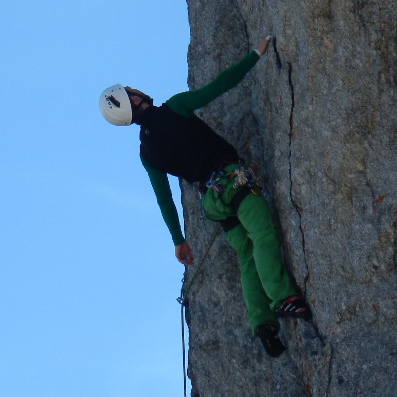
\includegraphics[height=3.5cm]{img/matthias.png}
		\end{column}
	\end{columns}
\end{frame}

\begin{frame}
\frametitle{Version 0.9 'Ganymede' (2007)}
	\begin{itemize}
		\item \textbf{Python bindings - This is the major focus of this release
			it is now possible to create plugins using python. It is also
			possible to create GIS enabled applications written in python 
			that use the QGIS libraries.}
		\item Removed automake build system - QGIS now needs CMake for compilation.
		\item Many new GRASS tools added (with thanks to http://faunalia.it/)
		\item Map Composer updates
		\item Crash fix for 2.5D shapefiles
		\item The QGIS libraries have been refactored and better organised.
		\item Improvements to the GeoReferencer
	\end{itemize}
\end{frame}

\begin{frame}
\frametitle{Plugin ecosystem}
	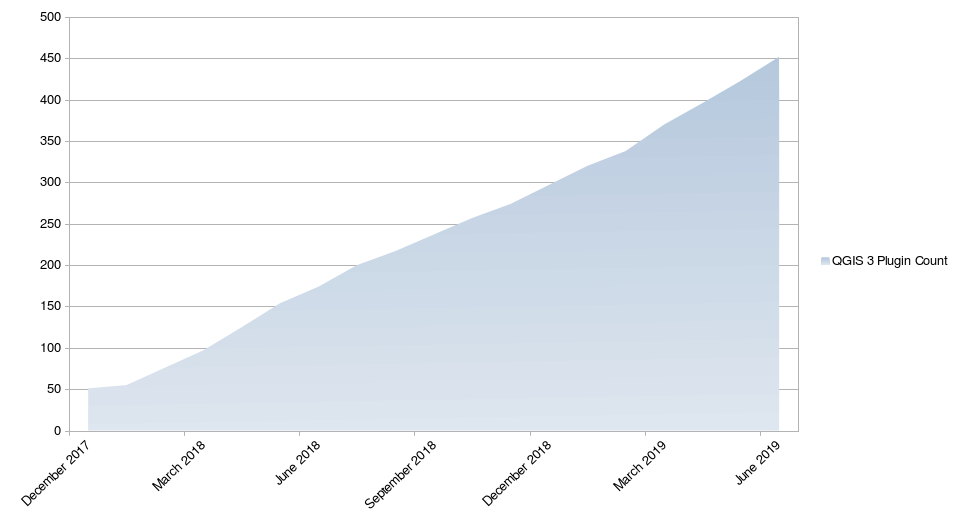
\includegraphics[width=0.9\textwidth]{img/qgis_plugin_count.png}
\end{frame}

\begin{frame}
\frametitle{Optimizing PyQGIS}

\begin{itemize}
	\item Various collections of "common pyqgis helper functions" have been written to "make things easier".
\end{itemize}

See: \url{http://osgeo-org.1560.x6.nabble.com/QGIS-Developer-Common-PyQGIS-functions-for-QGIS-3-td5395644.html}
\end{frame}

\begin{frame}
\frametitle{Common PyQGIS functions for QGIS 3}
\epigraph{``Wouldn't it be possible to provide such a collection of common pyqgis functions not only from private persons/projects but from the QGIS-project itself so users could add common functions?
I think the chances would be higher that such a "official" collection would be used in the long run and constantly extended."}{--- Thomas Baumann, QGIS Developer Mailing List}
\end{frame}

\begin{frame}
\frametitle{The goal}
\begin{description}
	\item [API first] Make flexible and easy to use APIs. Benefits Python and C++.
	\item [Pythonic] Implement ``Pythonic" constructs. Leverage modern Python language features.
\end{description}
\end{frame}
	\section{Decorators}


\subsection{Decorators}
\begin{frame}
\frametitle{Decorators}
	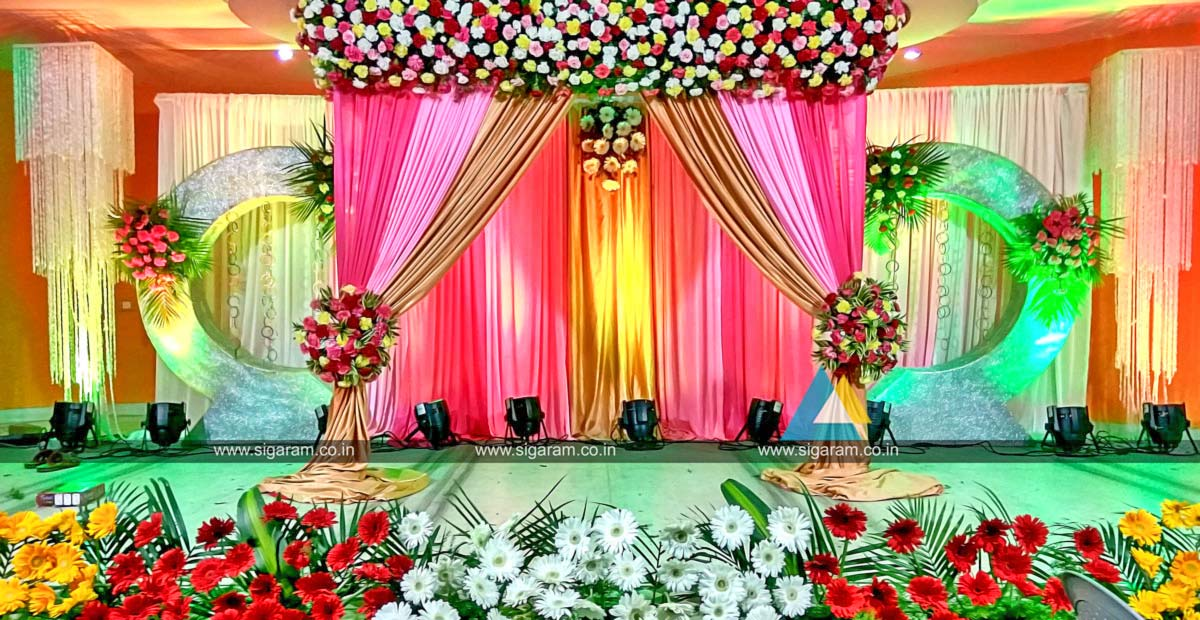
\includegraphics[width=0.9\textwidth]{img/decorators.jpg}
\end{frame}

\subsection{Decorators}
\begin{frame}
\frametitle{What is a Decorator}
\setlength{\epigraphwidth}{0.9\textwidth}
\epigraph{``A decorator is the name used for a software design pattern.
Decorators dynamically alter the functionality of a function, method, or class without having to directly use subclasses or change the source code of the function being decorated."}{--- https://wiki.python.org/moin/PythonDecorators}

\end{frame}

\subsection{Decorators}
\begin{frame}
\frametitle{A simpler explanation}
Decorators help to write code that is easier to write and read. It helps to avoid repeating "boilerplate code".

It's \emph{syntactic sugar}.
\end{frame}


\subsection{Expressions}
\begin{frame}[fragile]
\frametitle{Expression functions}
\begin{lstlisting}[style=pythoncode]
@qgsfunction(args='auto', group='Custom')
def sum(value1, value2, feature, parent):
    """
    Calculates the sum of the two parameters value1 and value2.
    <h2>Example usage:</h2>
    <ul>
      <li>my_sum(5, 8) -> 13</li>
      <li>my_sum("field1", "field2") -> 42</li>
    </ul>
    """
    return value1 + value2
\end{lstlisting}
\end{frame}

\subsection{Processing}
\begin{frame}
\frametitle{Processing}
	\begin{columns}[T] % contents are top vertically aligned
		\begin{column}[T]{7cm} % each column can also be its own environment
			\begin{itemize}
				\item Modular data processing pipelines
				\item Less effort to create the GUI
				\item But: A lot of boilerplate code
				\begin{itemize}
					\item Processing provider
					\item Methods for input and output definition
					\item Methods for help
					\item Method for the algorithm itself
				\end{itemize}
			\end{itemize}
		\end{column}
		\begin{column}[T]{3cm} % alternative top-align that's better for graphics
			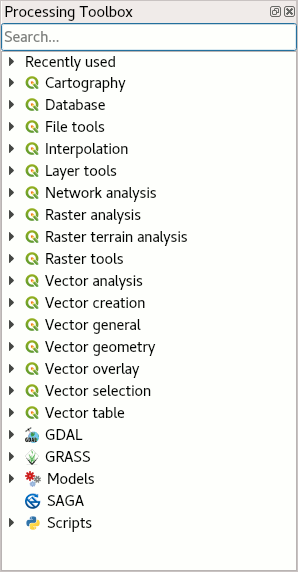
\includegraphics[height=7cm]{img/processing-toolbox.png}
		\end{column}
	\end{columns}
\end{frame}

\subsection{Processing}
\begin{frame}[fragile]
\frametitle{Processing Algorithm}
\begin{lstlisting}[style=pythoncode]
class GeoCoding(Algorithm):
	INPUT: 'INPUT'
	OUTPUT: 'OUTPUT'
	COLUMN_PREFIX: 'COLUMN_PREFIX'
	
	def name(self):
		return 'geocoding'
		
	def initAlgorithm(self, config=None):
		self.addParameter(
            QgsProcessingParameterFeatureSource(
                self.INPUT,
                self.tr('Address Layer')
            )
        )
	def displayName(self):
	def group(self):
	def shortHelpString(self):
	...
\end{lstlisting}
\end{frame}

\subsection{Processing}
\begin{frame}[fragile]
\frametitle{processing.alg decorator}
\begin{lstlisting}[style=pythoncode]
@alg(name="geocode", label=alg.tr("GeoCode"))
@alg.input(type=alg.SOURCE, name="INPUT", label="Adress layer")
@alg.input(type=alg.SINK, name="OUTPUT", label="Output layer")
def geocode(instance, parameters, context, feedback, inputs):
    """
    Geocode locations. Addresses in, points out.
    May produce multiple points for an address if ambiguous.
    """
	source = instance.parameterAsSource(parameters, "INPUT", context)
	(sink, dest\_id) = instance.parameterAsSink(parameters, "OUTPUT", context, source.fields(), QgsWkbTypes.Point, QgsCoordinateReferenceSystem(4326))

	GeoCoder.resolve(source, sink)
	
	return {"OUTPUT": dest\_id}
\end{lstlisting}
\end{frame}

\subsection{Processing}
\begin{frame}[fragile]
\frametitle{processing.alg decorator}
\begin{lstlisting}[style=pythoncode]
@alg(name="geocode", label=alg.tr("GeoCode"))
\end{lstlisting}

\end{frame}


\subsection{Validity checks}
\begin{frame}[fragile]
\frametitle{Validity checks}
\begin{lstlisting}[style=pythoncode]
@check.register(type=QgsAbstractValidityCheck.TypeLayoutCheck)
def layout_map_crs_choice_check(context, feedback):
	layout = context.layout
	results = []
	for i in layout.items():
		if isinstance(i, QgsLayoutItemMap) and i.crs().authid() == 'EPSG:3857':
			res = QgsValidityCheckResult()
			res.type = QgsValidityCheckResult.Warning
			res.title='Map projection is misleading'
			res.detailedDescription='The projection for the map item {} is set to <i>Web Mercator (EPSG:3857)</i> which misrepresents areas and shapes. Consider using an appropriate local projection instead.'.format(i.displayName())
			results.append(res)

		return results
\end{lstlisting}
\end{frame}

	\section{Exceptions}

\subsection{Handling exceptions}

\begin{frame}
\frametitle{When things go wrong}
	
\includegraphics[width=0.9\textwidth]{img/calvin.png}
\end{frame}

\subsection{Converting a geometry to a point}
\begin{frame}[fragile]
\frametitle{Converting a geometry to a point}

\begin{lstlisting}[style=pythoncode]
QgsGeometry.fromWkt('POINT(3 4)').asPoint()
\end{lstlisting}
\pause
\begin{lstlisting}[style=pythonoutput]
<QgsPointXY: POINT(3 4)>
\end{lstlisting}

\end{frame}

\subsection{Converting a geometry to a point}
\begin{frame}[fragile]
\frametitle{Converting a geometry to a point}

\begin{lstlisting}[style=pythoncode]
QgsGeometry.fromWkt('LINESTRING((3 4), (7 8))').asPoint()
\end{lstlisting}
\pause
\begin{lstlisting}[style=pythonoutput]
<QgsPointXY: POINT(0 0)>
\end{lstlisting}
\pause
... only until QGIS 3.4
\end{frame}

\subsection{Converting a geometry to a point}
\begin{frame}[fragile]
\frametitle{Converting a geometry to a point}

\begin{lstlisting}[style=pythoncode]
QgsGeometry.fromWkt('LINESTRING((3 4), (7 8))').asPoint()
\end{lstlisting}
\pause
\begin{lstlisting}[style=pythonoutput]
Traceback (most recent call last):
  File "plugins/somewhere/plugin.py", 
               line 90, in broken_method
TypeError: LineString geometry cannot be converted
           to a point. Only Point types are permitted.
\end{lstlisting}
\end{frame}

\subsection{When things go wrong}
\begin{frame}[fragile]
\frametitle{When things go wrong}

\begin{lstlisting}[style=pythoncode]
mp = QgsMultiPoint()
mp.addGeometry(QgsPoint(1,1))
mp.addGeometry(QgsPoint(2,2))
\end{lstlisting}
\pause
\begin{lstlisting}[style=pythoncode]
mp.geometryN(3)
\end{lstlisting}
\pause
\begin{lstlisting}[style=pythonoutput]
IndexError: 3
\end{lstlisting}

\end{frame}


\subsection{When things go wrong}
\begin{frame}[fragile]
\frametitle{When things go wrong}

\begin{lstlisting}[style=pythoncode]
try:
	mp.geometryN(3)
except IndexError as e:
	show_error(self.tr('The geometry is too short. Input data linestrings need to have at least 4 vertices.'))
\end{lstlisting}

\end{frame}


\subsection{Handling exceptions}

\begin{frame}
\frametitle{When things go wrong}
	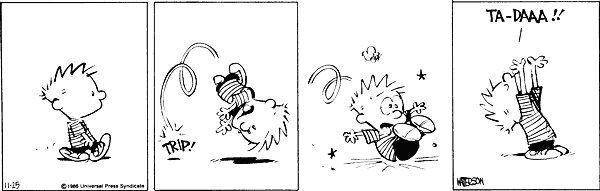
\includegraphics[width=0.9\textwidth]{img/calvin2.png}
\end{frame}
	\section{Atomic Operations}

\subsection{Atomic Operations}
\begin{frame}
\frametitle{Atomic Operations}
	
\includegraphics[width=0.9\textwidth]{img/atom.jpg}
\end{frame}


\subsection{Atomic operations using with}
\begin{frame}[fragile]
\frametitle{Atomic operations using with}

\begin{lstlisting}[style=pythoncode]
# Fix population from absolute to relative
layer.startEditing()
for feat in layer.getFeatures():
	feat['population'] = feat['population'] / feat['area']
	layer.updateFeature(feat)
layer.commitChanges()
layer.stopEditing()
\end{lstlisting}
\pause
\begin{lstlisting}[style=pythonoutput]
ZeroDivisionError: division by zero
\end{lstlisting}

\end{frame}

\subsection{Atomic Operations}
\begin{frame}
\frametitle{Atomic Operations}
	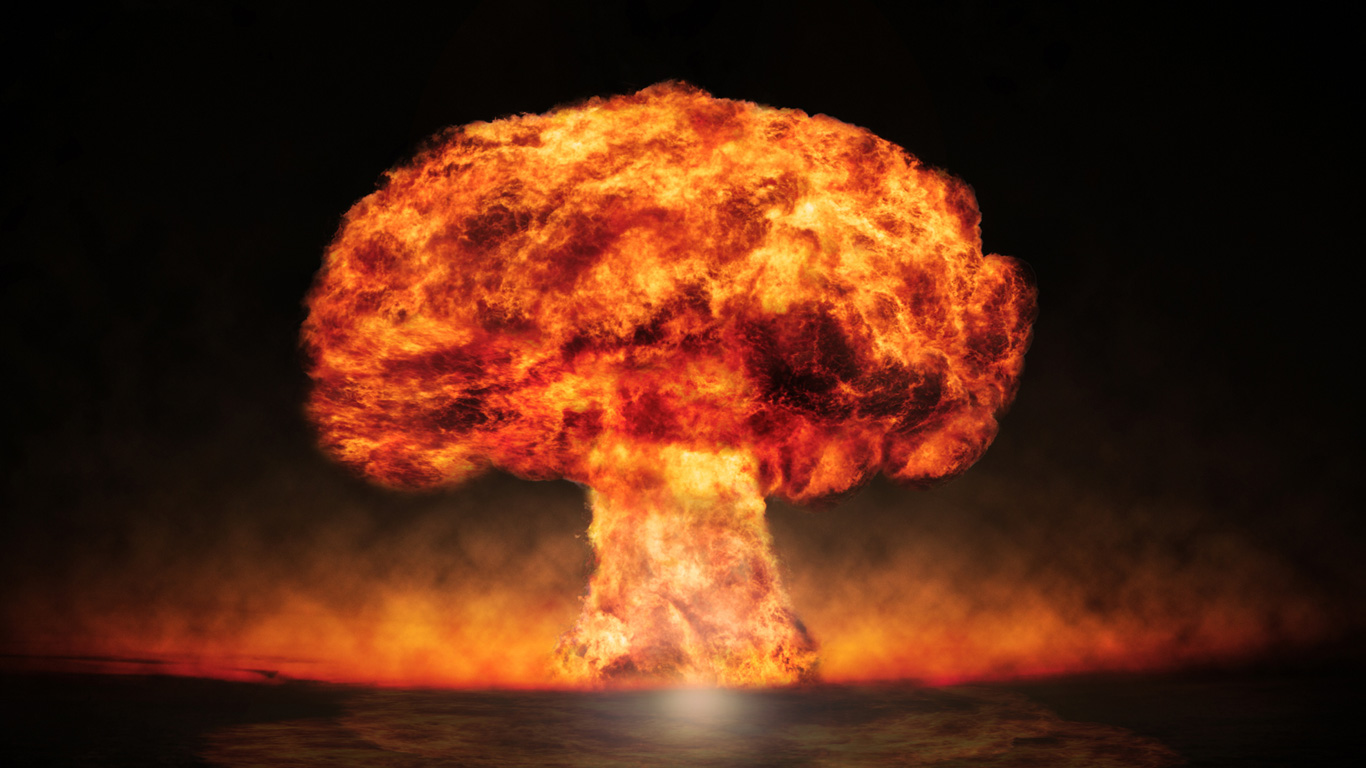
\includegraphics[width=0.9\textwidth]{img/atombombe.jpg}
\end{frame}

\subsection{Atomic operations using "with"}
\begin{frame}[fragile]
\frametitle{Atomic operations using "with"}
\begin{itemize}
	\item Only part of the features are modified
	\item The layer may or may not be in edit state any more
\end{itemize}
\end{frame}

\subsection{Atomic operations using "with"}
\begin{frame}[fragile]
\frametitle{Atomic operations using "with"}
Let's introduce "with"
\end{frame}

\subsection{Atomic operations using "with"}
\begin{frame}[fragile]
\frametitle{Atomic operations using "with"}

\begin{lstlisting}[style=pythoncode]
# Fix population from absolute to relative
with edit(layer):
	for feat in layer.getFeatures():
		feat['population'] = feat['population'] / feat['area']
		layer.updateFeature(feat)
# Changes are committed automatically if no error occurred
\end{lstlisting}
\pause
\begin{lstlisting}[style=pythonoutput]
# Or if an error occurs, no changes are applied at all
ZeroDivisionError: division by zero
\end{lstlisting}

\end{frame}

\subsection{Atomic Operations}
\begin{frame}
\frametitle{Atomic Operations}
	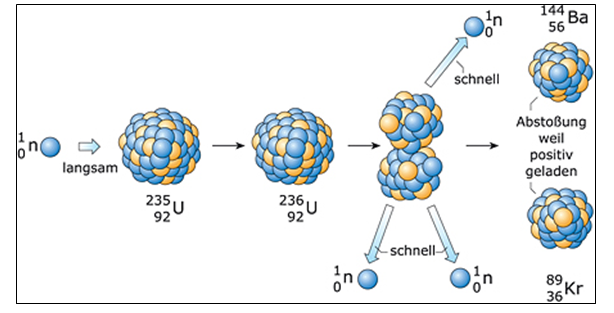
\includegraphics[width=0.9\textwidth]{img/controlled-chain-reaction.png}
\end{frame}

	\section{Iterators}

\subsection{Iterators}

\begin{frame}
\frametitle{Working with geometries}
	
\includegraphics[width=0.7\textwidth]{img/geometries.jpg}
\end{frame}

\subsection{Iterating vertices}
\begin{frame}[fragile]
\frametitle{Iterating vertices}

\begin{lstlisting}[style=pythoncode]
line = QgsGeometry.fromWkt('LINESTRING(1 1, 2 2)')
for vertex in line.vertices():
	print(vertex)
\end{lstlisting}
\pause
\begin{lstlisting}[style=pythonoutput]
<QgsPoint: Point (1 1)>
<QgsPoint: Point (2 2)>
\end{lstlisting}

\end{frame}

\subsection{Iterating parts}
\begin{frame}[fragile]
\frametitle{Iterating parts}

\begin{lstlisting}[style=pythoncode]
multipoint = QgsGeometry.fromWkt('MULTIPOINT((1 1), (2 2), (3 3))')
for point in multipoint.parts():
	print(point)
\end{lstlisting}
\pause
\begin{lstlisting}[style=pythonoutput]
<QgsPoint: Point (1 1)>
<QgsPoint: Point (2 2)>
<QgsPoint: Point (3 3)>
\end{lstlisting}

\end{frame}

	\subsection{Representing objects}
\begin{frame}[fragile]
\frametitle{Representing objects}

\begin{lstlisting}[style=pythoncode]
QgsPoint(2635450,1244252)
\end{lstlisting}
\pause
\begin{lstlisting}[style=pythonoutput]
<qgis._core.QgsPoint object at 0x7fcd2b428ee8>
\end{lstlisting}

\end{frame}

\subsection{Representing objects}
\begin{frame}[fragile]
\frametitle{Representing objects, Since QGIS 3.2}

\begin{lstlisting}[style=pythoncode]
QgsPoint(2635450,1244252)
\end{lstlisting}
\pause
\begin{lstlisting}[style=pythonoutput]
<QgsPoint: Point (2635450 1244252)>
\end{lstlisting}

\end{frame}

	\section{Outlook}


\subsection{}
\begin{frame}
\frametitle{Outlook}
	
\includegraphics[width=0.9\textwidth]{img/plan.png}
\end{frame}

\subsection{Exception handling}
\begin{frame}
\frametitle{Exception handling}
\begin{itemize}
	\item Exceptions are good
	\begin{itemize}
		\item Exceptions help to fix problems
		\item Exceptions help in case of data corruption	
	\end{itemize}
	\item More exceptions
	\item E.g. instead of return values
\end{itemize}
\end{frame}

\subsection{Easier initialization}
\begin{frame}
\frametitle{Easier initialization}
\begin{itemize}
	\item A lot of boilerplate code is required to get started with a standalone application
	\item Goal: reduce that
\end{itemize}
\end{frame}

\subsection{More pythonic constructs}
\begin{frame}
\frametitle{More pythonic constructs}
\begin{itemize}
	\item More decorators
	\item More iterators
\end{itemize}
\end{frame}

\subsection{Nice API}
\begin{frame}
\frametitle{Nice API}
\begin{itemize}
	\item But that is not Python specific
\end{itemize}
\end{frame}

\subsection{Start Coding}
\begin{frame}
\frametitle{Start Coding}
	\begin{columns}[T] % contents are top vertically aligned
		\begin{column}[T]{5cm} % each column can also be its own environment
		\begin{itemize}
			\item Let's get to work
		\end{itemize}
		\end{column}
		\begin{column}[T]{5cm} % alternative top-align that's better for graphics
			
\includegraphics[height=3.5cm]{img/start_coding.jpg}
		\end{column}
	\end{columns}
\end{frame}

\subsection{Thank you}
\begin{frame}
\frametitle{Thank you}
Questions?
Now or later...
\end{frame}

\end{document}
